\chapter{High-pass and low-pass filters} \label{chap:high_low}
The theory in this chapter is based on \cite{bcircuit}\cite{bcircuit5}.\\
The main purpose of high-pass and low-pass filters is to remove unwanted frequencies from a signal. Filters are often used on sound files to control the bass and treble. There are different kinds of filters that can remove unwanted frequencies. This section focuses on high and low-pass filters.

\section{Definitions}
In this section the most central terms concerning high-pass and low-pass filters will be defined. The definitions are essential when understanding the most important derivations in section \ref{Derivations}.

\subsection{Low-pass filters}
A low-pass filter passes frequencies from  $0~Hz$ to a certain cut-off frequency, after which the amplitude of the signal is decreased.  
\\
In the illustration below, the voltage output is measured across the capacitor, which decreases the high frequencies, and leaves the low frequencies unchanged.
\\
\begin{figure}[H]
	\begin{center}
\begin{circuitikz}[american voltages]
\draw (0,0)
to[sqV, sqV=$V_{AC}$] (0,2)
to (6,2)
to[short, -] (4,2)
to[C=$C$] (4,0)
to (6,0)
to (4,0)
to [resistor, R=$R$] (0,0);
\draw [>=latex', <->] (6,1.75) -- node[anchor=west] {$V_{output}$} (6,0.25);
\end{circuitikz}
\end{center}

	\caption{Circuit diagram of a low-pass filter.} \label{lp:diagram}
\end{figure} 
\subsection{High-pass filters}
High-pass filters are in many ways similar to the low-pass filters. A high-pass filter cuts off frequencies below a certain cut-off frequency. \\
The voltage output is measured across the resistor ($R$) instead of the capacitor ($C$). 
\begin{figure}[H]
	\begin{center}
\begin{circuitikz}[american voltages]
\draw (0,0)
to[sV, sV=$V_{AC}$] (0,2)
to (6,2)
to[short, -] (4,2)
to[resistor, R=$R$] (4,0)
to (6,0)
to (4,0)
to [C=$C$] (0,0);
\draw [>=latex', <->] (6,1.75) -- node[anchor=west] {$V_{output}$} (6,0.25);
\end{circuitikz}
\end{center}

	\caption{Circuit diagram of a high-pass filter.}
	\label{hp:diagram}
\end{figure} 

\subsection{Cut-off frequencies}
(The cut-off frequency for a low-pass filter is the frequency at which the bode plot is decreased by $3\ dB$, and for a high-pass filter it is when the bode plot is $3dB$ away from reaching zero). The cut-off frequency is also the frequency, where the filtering (both high- and low-pass filters) starts getting efficient. The definition of a cut-off frequency is when the effect is halved. The amount of decibel can be calculated as follows: \cite[p. 596-597]{bcircuit}
\begin{align} \label{number:db}
Gain = 10 \log \left(\dfrac{P_{output}}{P_{input}} \right).
\end{align}
The point at which the effect is halved, is when $\dfrac{P_{output}}{P_{input}}$ is equal to $\dfrac{1}{2}$. The gain of negative $3\ dB$ is inserted into \eqref{number:db}:
\begin{align*} 
10 \log \left(\dfrac{1}{2} \right) = -3 dB.
\end{align*}
From \eqref{resistor:power}, the effect, $P$, is defined as $P=\dfrac{v^2}{R}$:
\begin{align*}
Number \ of \ dB = 10 \log \left(\dfrac{\dfrac{v_{output}^2}{R}}{\dfrac{v_{input}^2}{R}} \right).
\end{align*}
This can be simplified:
\begin{align} \label{number:db:volt}
Number \ of \ dB = 10 \log \left(\left(\dfrac{v_{output}}{v_{input}} \right)^2\right).
\end{align}
From \eqref{number:db} and \eqref{number:db:volt}, the following relation can be derived: $$\dfrac{P_{output}}{P_{input}}= \left(\dfrac{v_{output}}{v_{input}} \right)^2$$ To find the point at which the power is halved, the right side of the above equation can be set equal to $\dfrac{1}{2}$:
\begin{align*}
\dfrac{1}{2}= \left(\dfrac{v_{output}}{v_{input}} \right)^2.
\end{align*}
This can be simplified:
\begin{align} \label{eq:v_ratio}
\dfrac{1}{\sqrt{2}}= \dfrac{v_{output}}{v_{input}}.
\end{align}
From \eqref{eq:v_ratio}, it is found that the amplitude is decreased by $1-\left(\dfrac{1}{\sqrt{2}} \right) = 29.3\%$. 
\\
The gain of the signal can also be defined in terms of the input and output signals. Equation \eqref{number:db:volt} can be rewritten as:
\begin{align*}
	Gain =& 10 \log \left(\left(\dfrac{v_{output}}{v_{input}} \right)^2\right),
	\\
	     =& 20 \log \left(\dfrac{v_{output}}{v_{input}} \right).
\end{align*}
The relevance of this will become apparent in subsection \ref{sub:TTF}.

\subsection{Bode plots} \label{sub:bode}
Bode plots are two separate graphical representations of the magnitude response (also called the gain) and phase response of a system with respect to frequency. They are especially useful in analysing frequency-dependent systems and networks such as filters, tuners, and amplifiers. \cite [p. 626]{bcircuit5}  \\
\\
The magnitude response is plotted in a coordinate system with a logarithmic $x$-axis. For a low-pass filter, the output wave before the cut-off point will remain almost unchanged. Above the cut-off point, the output decreases by $20\ dB$ per decade compared to the input, and the amplitude decreases and approaches a graph similar to that of DC current. \\
The bode magnitude plot for a high-pass filter starts in negative decibel and approaches zero. Until it reaches the cut-off point, the graph increases with $20\ dB$ per decade. When reaching the cut-off point, the graph is $3 \ dB$ less than the input signal.

\subsection{The imaginary angular frequency}
The experiment in chapter \ref{chap:RC} for testing the capacitor used a DC voltage. In the case of high and low pass filters, a sinusoidal input will be applied. The voltage, in this case, can be written as a wave function:
\begin{align*}
v(t)=A\sin(\omega_f t+\theta),
\end{align*}
where $A$ is the amplitude, $\omega_f=2\pi f$, and $\theta$ is the phase shift. For the purpose of this experiment, the phase shift of the input signal will not be considered. According to definition \ref{lpdef}, $s=\sigma + i \omega$. If the real part is set to zero ($\sigma = 0$), $i \omega$ is considered the imaginary angular frequency. $s$ can then be rewritten as $s = i \omega_f$. \cite[p. 733 - 735]{bcircuit9}

\subsection{The transfer function} \label{sub:TTF}
The transfer function describes what happens to an input signal, when it is sent through a system. The transfer function is denoted as $H(s)$.
\\
\begin{figure}[H]
\center
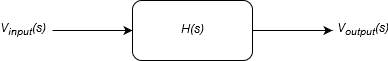
\includegraphics[scale=0.6]{fig/img/transfer_function.png}
\caption{A voltage input is sent through a system, and the output is the response to the transfer function}
\label{fig:transfer}
\end{figure}
\noindent
The signal output can be described in terms of the signal input and the transfer function.
\begin{align*}
V_{output}(s)=V_{input}(s)H(s),
\end{align*}
where $V_{output}(s)=\mathcal{L}\{v_{output}(t)\}$, and $V_{input}(s)=\mathcal{L}\{v_{input}(t)\}$

\section{Derivations} \label{Derivations}
In the following section, the transfer function for low-pass and high-pass filters are derived, as well as the cut-off frequencies for both filters.

\subsection{Transfer function for low-pass filters}
Consider \eqref{eq:dvC(t)}:
\begin{align} \label{eq:dV_C}
\dfrac{dv_C(t)}{dt}=-v_R(t)\dfrac{1}{RC}.
\end{align}
From KVL, the algebraic sum of voltages can be written as: 
\begin{align}
v_{input}(t)-v_{R}(t)+v_{C}(t)=0,\nonumber
\\
\Leftrightarrow -v_{R}(t) = v_{input}(t) - v_{C}(t). \label{eq:KVL_low}
\end{align}
\eqref{eq:KVL_low} is inserted in \eqref{eq:dV_C}:
\begin{align*} 
\dfrac{dv_C(t)}{dt}&=\Big(v_{input}(t) - v_{C}(t)\Big)\dfrac{1}{RC},
\\
&=\dfrac{1}{RC}v_{input}(t) - \dfrac{1}{RC}v_{C}(t).
\end{align*}
$\dfrac{1}{RC}v_C(t)$ is added to both sides:
\begin{align*}
\dfrac{dv_C(t)}{dt}+\dfrac{1}{RC}v_C(t)=\dfrac{1}{RC}v_{input}(t).
\end{align*}
This differential equation can now be solved using the Laplace transform:
\begin{align}\label{eq:laplace:low}\mathcal{L}\bigg\{\dfrac{dv_C(t)}{dt}\bigg\}+\dfrac{1}{RC}\mathcal{L}\Big\{v_C(t)\Big\}=\dfrac{1}{RC}\mathcal{L}\Big\{v_{input}(t)\Big\}.
\end{align}
According to \cref{theorem:lap_diff}, \eqref{eq:laplace:low} yields the following equation:
\begin{align*}
V_C(s)s+v_C(0)+\dfrac{1}{RC}V_C(s)=\dfrac{1}{RC}V_{input}(s).
\end{align*} 
$v_{C}$ is now factorised, and the initial voltage across the capacitor is zero, which can be derived from \eqref{V_up}:
\begin{align*}
\dfrac{1}{RC}V_{input}(s)=V_{C}(s)\Big(\dfrac{1}{RC}+s\Big).
\end{align*} 
The ratio of the voltages is isolated:
\begin{align*}
\dfrac{\dfrac{1}{RC}}{\dfrac{1}{RC}+s} = \dfrac{V_{C}(s)}{V_{input}(s)}=H_L(s).
\end{align*}
It would now be interesting to see how the ratio between input and output responds to different frequencies. To do this, the previously defined $s$ as $s=i\omega_f$ is used:
\begin{align} \label{eq:trans_low}
H_{L}(i \omega_f) = \dfrac{\dfrac{1}{RC}}{\dfrac{1}{RC}+i \omega_f}. 
\end{align}
Both sides of the equation are multiplied by $\dfrac{RC}{RC}$:
\begin{align*}
H_{L}(i \omega_f) = \dfrac{RC}{RC} \cdot \dfrac{\dfrac{1}{RC}}{\dfrac{1}{RC}+i \omega_f}. 
\end{align*}
This can be simplified:
\begin{align*}
H_{L}(i \omega_f) =  \dfrac{1}{1+RC \cdot i \omega_f}. 
\end{align*}
From \eqref{eq:v_ratio}, it can be concluded that the cut-off frequency occurs, when the amplitude of the output is $\dfrac{1}{\sqrt{2}}$ of the input. Using \eqref{eq:mod_div}, modulus of the transfer function is found:
\begin{align}
\left|H_{L}(i \omega_f) \right| &=  \left|\dfrac{1}{1+RC \omega_f} \right|, \nonumber
\\
&=\dfrac{|1|}{|1+RC\omega_f |}, \nonumber
\\
&=  \dfrac{1}{\sqrt{1+(RC \omega_f)^2}}. \label{tf:mod}
\end{align}
\textbf{Deriving the cut-off frequency for a low-pass filter}\\
Equation \eqref{tf:mod} describes the relation between the amplitude of the input and the output signal. This expression is set equal to $\dfrac{1}{\sqrt{2}}$, and the frequency is found:
\\
\begin{align*}
\dfrac{1}{\sqrt{1+ \left(RC \cdot \omega_f \right)^2}} = \dfrac{1}{\sqrt{2}}.
\end{align*}
Both sides are squared:
\begin{align*}
\dfrac{1}{1+ \left(RC \cdot \omega_f \right)^2} = \dfrac{1}{2}.
\end{align*}
	Both sides are multiplied by $2(1+(RC\omega_f)^2)$:
\begin{align*}
2 = 1+ \left(RC \cdot \omega_f \right)^2.
\end{align*}
Both sides are subtracted by 1, and then raised to the power of $\dfrac{1}{2}$:
\begin{align*}
1 = RC \cdot \omega_f .
\end{align*}
Note that from equation \eqref{eq:omega}, $\omega_f$ is defined as $\omega_f=2 \pi f$:
\begin{align*}
1 = RC 2\pi f .
\end{align*}
Now $f$ is isolated:
\begin{align*}
f=\dfrac{1}{2\pi RC}.
\end{align*}
The cut-off frequency of the circuit is then defined.

\subsection{Transfer function for high-pass filters}
Similarly, the transfer function is derived from equation \eqref{eq:dvC(t)} :
\begin{align*}
\dfrac{dv_{C}(t)}{dt} = -v_{R}(t) \cdot \dfrac{1}{RC}.
\end{align*}
Firstly, both sides are multiplied by $-RC$:
\begin{align*}
-RC \cdot \dfrac{dv_{C}(t)}{dt} = v_{R}(t).
\end{align*}
Since it is now a high-pass filter (and a different circuit), KVL has to be rewritten and is now $v_{C}(t)=v_{R}(t)-v_{input}(t)$. Both sides of this expression are now differentiated, and can be inserted on the left-hand side above:
%den ovensående sætning lyder mærkelig, er de begge differetieret eller er de differentiable?
\begin{align*}
-RC \cdot \left(\dfrac{dv_{R}(t)}{dt} - \dfrac{dv_{input}(t)}{dt} \right) = v_{R}(t).
\end{align*}
The Laplace transform is now applied to both sides of the equation:
\begin{align*}
-RC \mathcal{L} \left\{\dfrac{dv_{R}(t)}{dt} \right\} + RC \mathcal{L} \left\{ \dfrac{dv_{input}(t)}{dt} \right\} = \mathcal{L} \left\{v_{R}(t) \right\}.
\end{align*}
The values can be found from table \ref{lptable} in the previous chapter:
\begin{align*}
-RC \big(sV_{R}(s)-v_{R}(0)\big) + RC \left(sV_{input}(s)-v_{input}(0)\right) = V_{R}(s).
\end{align*}
It is assumed that $v_{R}(0)$ and $v_{input}(0)$ are both equal to zero:
\begin{align*}
-RCsV_{R}(s) + RCsV_{input}(s) = V_{R}(s).
\end{align*}
Now $RCs V_{input}(s)$ is isolated:
\begin{align*}
RCsV_{input}(s) = V_{R}(s) + RCsV_{R}(s).
\end{align*}
$V_{R}(s)$ is factorised:
\begin{align*}
RCsV_{input}(s) = V_{R}(s) \cdot (1 + RCs).
\end{align*}
The ratio of the voltages is isolated:
\begin{align} \label{hp:visolated}
\dfrac{RCs}{1 + RCs} = \dfrac{V_{R}(s)}{V_{input}(s)}.
\end{align}
Note, that $s=i\omega_f$. The equation can then be rewritten as:
\begin{align*}
H_{H}(i \omega_f) = \dfrac{RCi \omega_f}{1 + RCi \omega_f}.
\end{align*}
To find the cut-off frequency, modulus of the transfer function is found:
\begin{align}
\left|H_{H}(i \omega_f)\right| &= \left|\dfrac{RCi \omega_f}{1 + RCi \omega_f} \right|, \nonumber \\
 &= \dfrac{|RCi \omega_f|}{|1 + RCi \omega_f |}, \nonumber \\
 &= \dfrac{\sqrt{(RC \omega_f)^2}}{\sqrt{1 + (RC \omega_f)^2 }}, \nonumber \\
 &= \dfrac{RC \omega_f}{\sqrt{1 + (RC \omega_f)^2 }}. \label{tfmodhp}
\end{align} 
\textbf{Deriving the cut-off frequency for a high-pass filter} \\
This expression is set equal to $\dfrac{1}{\sqrt{2}}$:
\begin{align*}
\dfrac{RC \omega_f}{\sqrt{1 + (RC \omega_f)^2 }}=\dfrac{1}{\sqrt{2}}.
\end{align*}
Both sides of the equation are squared:
\begin{align*}
\dfrac{(RC \omega_f)^2}{1 + (RC \omega_f)^2 }=\dfrac{1}{2}.
\end{align*}
Both sides are multiplied with $1+(RC\omega_f)^2$:
\begin{align*}
(RC \omega_f)^2 =\dfrac{1}{2}+\dfrac{1}{2}(RC\omega_f)^2.
\end{align*}
Both sides are subtracted  by $\dfrac{1}{2}(RC\omega_f)^2$:
\begin{align*}
\dfrac{1}{2}(RC \omega_f)^2 =\dfrac{1}{2}.
\end{align*}
Both sides are multiplied with $\dfrac{2}{(RC)^2}$:
\begin{align*}
\omega_f^2 =\dfrac{1}{(RC)^2}.
\end{align*}
Both sides of the equation are raised to the power of $\dfrac{1}{2}$:
\begin{align*}
\omega_f =\dfrac{1}{RC}.
\end{align*}
From equation \eqref{eq:omega}, $\omega_f$ is defined as $\omega_f=2 \pi f$:
\begin{align*}
2\pi f=&\dfrac{1}{RC},
\\
f=&\dfrac{1}{2\pi RC}.
\end{align*}

\noindent Equation \eqref{tfmodhp} describes the numerical relation between the input and output signal.


\section{Experiment} \label{experiment}
The following section conducts experiments with high- and low-pass filters, and examines the data. Similar to the transient analysis of the capacitor, the circuit is set-up using the Analog Discovery 2, and consists of a resistor and a capacitor. Additionally, the input voltage  is a  sinusoidal wave. \\
When testing the low-pass filter, the voltage across the capacitor is measured. When testing the high-pass filter, the voltage across the resistor is measured.

\subsection{Simulation of the circuit}
Simulated values are generated to test the data from the experiment. This is helpful when testing the validity of the test values. There are a couple of essential things to compare when testing the validity of a high- and low-pass filter, which are the cut-off frequency and coefficient of determination. 
\\ \\
The transfer functions derived from \cref{Derivations} were tested by using them to simulate a physical circuit. The circuits were set up as follows:
\\
\\
\textbf{Anders indsætter nogle lækrer graphics} 
\\
\\
The resistor in both circuits had a resistance of $4770 \Omega$, and the capacitor had a capacitance of $97.61\cdot 10^{-9} F$. The frequencies of the input-signal ranged from $1 Hz$ to $100,000 Hz$ in the case of the test for the high-pass filter. In the case of the low-pass filter, the frequencies ranged from $1 Hz$ to $1622165.753 Hz$.
\\
\\
Both of the simulations were created using the input data, which were also were used in the experiment. The input data were in units of hertz, which was converted to angular frequencies for the plot.
\\
The voltage gain of the input signal is defined as:
\begin{align*}
	gain_H(\omega _f) =&20 \cdot \log{\left( \left|H_{H}(i \omega_f)\right| \right)},
	\\
	gain_L(\omega _f) =&20 \cdot \log{\left( \left|H_{L}(i \omega_f)\right| \right)}.
\end{align*}

\noindent The input data was then fed into the functions. The relation between the input and output was then plotted on a graph with a linear y-axis, and logarithmic x-axis:

\begin{figure}[htbp]
\centering
	\begin{subfigure}[b]{0.49\textwidth}
		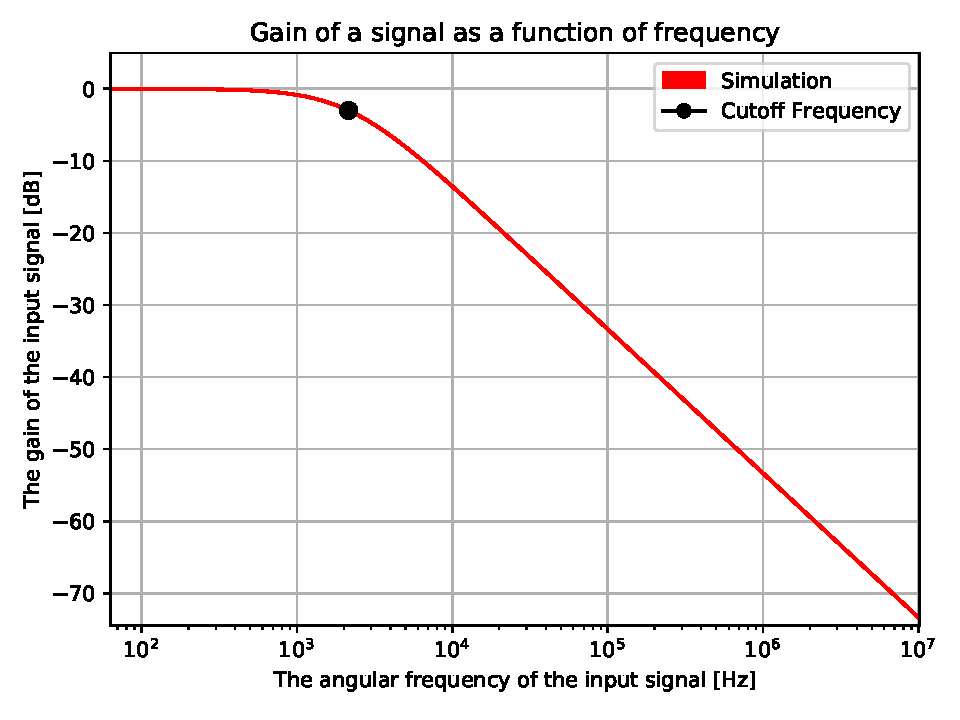
\includegraphics[width=\textwidth]{fig/img/LPF_sim.pdf}
    		\label{fig:lpf_sim}
    		\caption{Simulation of the low-pass filter}
	\end{subfigure}
	\begin{subfigure}[b]{0.49\textwidth}
		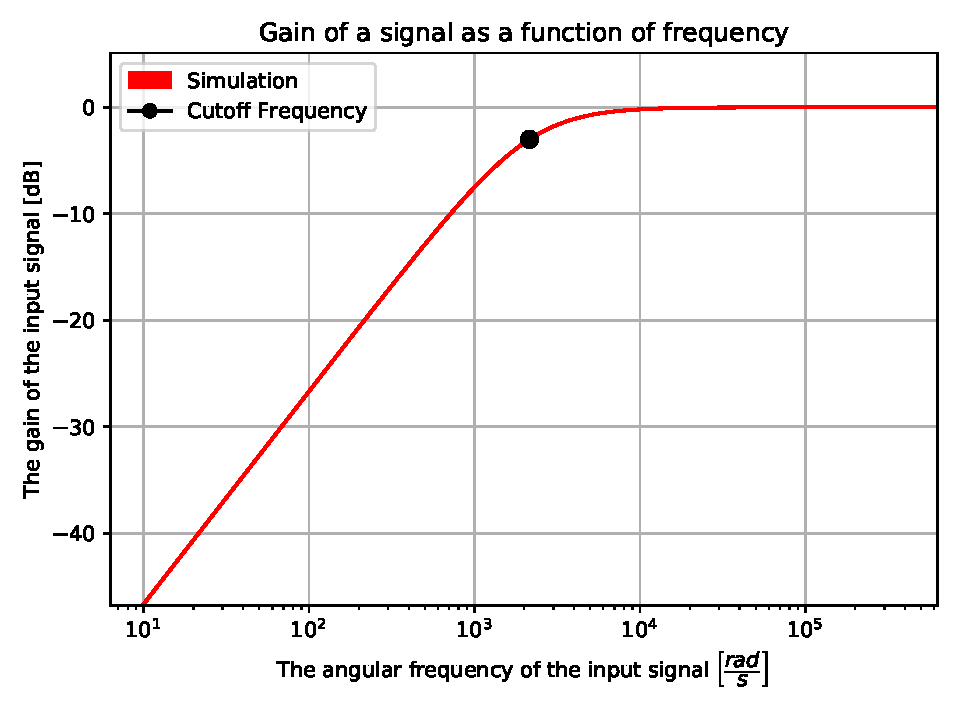
\includegraphics[width=\textwidth]{fig/img/HPF_sim.pdf}
    		\label{fig:hpf_sim}
    		\caption{Simulation of the high-pass filter}
	\end{subfigure}
\caption{Simulated bode magnitude plots for the high- and low-pass filters in the experiment.}
\end{figure}

\noindent Since the data and the simulation is plotted using angular frequency, the cut-off frequency must be converted to angular frequency as well:
\begin{align}
	\omega _c =& \dfrac{1}{RC2\pi} \cdot 2\pi = \dfrac{1}{RC}, \nonumber \\
			  =& \dfrac{1}{4770 \Omega \cdot 97.61 \cdot 10^{-9} F}, \nonumber \\
			  =& 2148 \dfrac{rad}{s}. \label{sim:cut}
\end{align}

\subsection{Test values}
The test values are generated using Analog Discovery 2 to set up the circuits. Figure \ref{rc_flow} shows the circuit for the charge and discharge of the capacitor. The same circuit is used to describe the low-pass filter. When setting up the circuit for a high-pass filter, the only change is that the voltmeter measures across the resistor instead of the capacitor. 
\\ \\ 
When plotting the data in the same bode plot as the simulated values, it is going to look as follows: \\
\begin{figure}[htbp]
\centering
	\begin{subfigure}[b]{0.49\textwidth}
		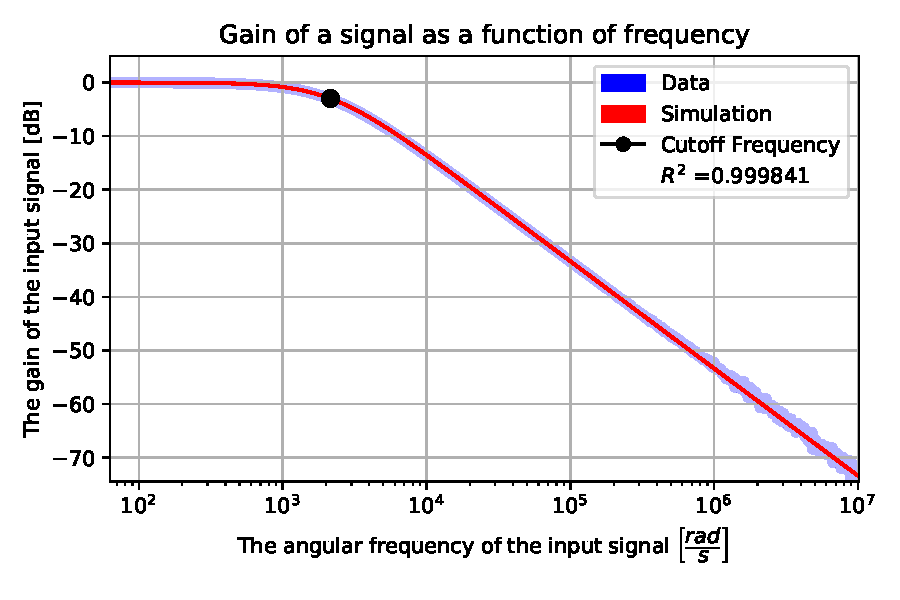
\includegraphics[width=\textwidth]{fig/img/LPF_exp.pdf}
    		\caption{Test values, simulation values, and the cut-off frequency for the low-pass filter}
    		\label{fig:lpf:exp}
	\end{subfigure}
	\begin{subfigure}[b]{0.49\textwidth}
		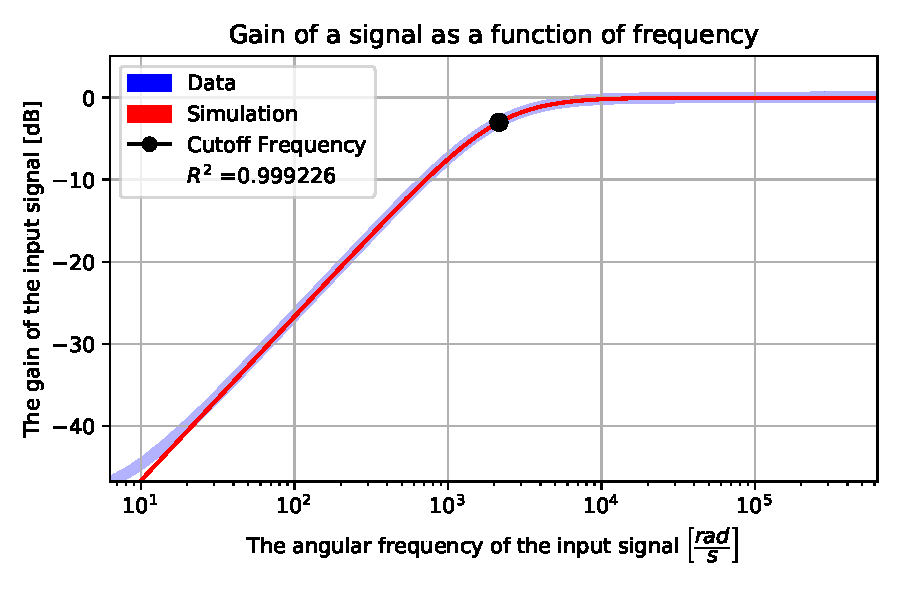
\includegraphics[width=\textwidth]{fig/img/HPF_exp.pdf}
    		\caption{Test values, simulation values, and the cut-off frequency for the high-pass filter}
    		\label{fig:hpf:exp}
	\end{subfigure}
	\caption{Test values for a low- and high-pass filter}
\end{figure}
\\ \\
The data is based on 1001 measuring points generated by Analog Discovery 2. From these 1001 measuring points on the bode plot, the one closest to the cut-off frequency is found to compare with the simulated cut-off value. The simulated cut-off value for low-pass filters is found to be $336.17 Hz$, and can be converted to $\dfrac{rad}{s}$:
\begin{align}
336.17 \cdot 2 \pi = 2112.22 \ \dfrac{rad}{s}.
 \label{lpf:cut}
\end{align}
Similarly, this can be found for the high-pass filter:
\begin{align}
342.77 \cdot 2 \pi = 2153.69 \ \dfrac{rad}{s}.
 \label{hpf:cut}
\end{align}
\subsection{Comparison}
In the following section, the test values for the low-pass filter and its simulated data are compared, followed by a comparison of the high-pass filters test values and its simulated data.
\\ \\
When observing figure \ref{fig:lpf:exp}, it becomes clear that the data from the experiment is almost identical to the simulated data. The coefficient of determination is almost equal to one, which underlines that the two functions are almost the same. Because the lower gain in decibel is more difficult to measure, the measuring points of the data become more inaccurate, as the angular frequency increases. As stated in section \ref{sub:bode}, the graph decreases by $20\ dB$ per decade after the cut-off point. Furthermore, the percentual difference between the simulated cut-off frequency versus the measured can be found, using the values in \eqref{sim:cut} and \eqref{lpf:cut}: $$1-\dfrac{2112.22\ \dfrac{rad}{s}}{2148\ \dfrac{rad}{s}}= 0.0167 = 1.67 \%.$$
\\ \\
The data from the high-pass filter shown in figure \ref{fig:hpf:exp} is close to the simulated data for the experiment. Moreover, when the frequency is $10^{1}$, the gain is approximately $-45\ dB$. When observing the next decade $10^{2}$, the gain is approximately $-25\ dB$. Therefore the bode plot corresponds with the increasing $20\ dB$ per decade, as stated in section \ref{sub:bode}. Now, the percentual difference between the simulated cut-off frequency  and the cut-off frequency measured from the data can be found: 
$$1-\dfrac{2153.69\ \dfrac{rad}{s}}{2148\ \dfrac{rad}{s}}= 0.0026 = 0.26 \%.$$
It can now be seen that the two cut-off frequencies are almost identical to the simulated cut-off frequencies.
\\ \\
From the comparisons on high- and low-pass filters it is now clear what the biggest source of error is. Both of the experimental graphs are aligned on top of the simulated graphs, at all outputs close to $0\ dB$. The further the output in decibel comes from 0, the more inaccurate the graphs are. Therefore the most relevant uncertainty in the experiment is the accuracy of the measuring instrument at a really low decibel output.